\chapter{Maximum Principle Exercise 1 mm3}

\assignment{
  Consider the one-dimensional continuous-time optimization problem:
  \begin{equation}
    \label{eq:max_eq1}
    \max_u\int_0^T -\frac{1}{2}\left( x^2 + u^2 \right)\,\up{dt}
  \end{equation}
  subject to:
  \begin{equation}
    \label{eq:max_eq2}
    \dot{x} = -\tanh{\left( x \right)} + u,\quad x(0) = x_0
  \end{equation}
  \begin{enumerate}
    \item Write the discrete-time version of \eqref{eq:max_eq1}. $\left( \text{Hint: use }\dot{x} = \frac{\Delta
          x_k}{\Delta t}\right)$
    \item Use the discrete maximum principle to write down the state- and costate equations.
    \item With $T = 4$, $x_0 = 5$ and $\Delta t = 1$, use matlab to solve the TPBVP (two point boundary value
      problem). (Hint: write a function with input$^1$ =``a guess on $\lambda_0$'' and output=``$\lambda_T$''. Then use
\texttt{fzero} on this function.)
  \end{enumerate}
~\\
  \footnotesize{$^1$try -0.2}
}

\assignment{1. Write the discrete-time version of \eqref{eq:max_eq1}. $\left( \text{Hint: use }\dot{x} = \frac{\Delta
      x_k}{\Delta t}\right)$:}

The objective function is integrated, this becomes a summation in discrete time. Furthermore $x(0) = x_0$,
this changes the lower limit of the summation. The objective function then becomes:
\begin{equation}
  \max_u\sum_{k = 1}^{T - 1} -\frac{1}{2}\left( x^2_k + u^2_k \right)\Delta t
\end{equation}
The equality constraint  are discretised using the hint given:
\begin{equation}
  \begin{split}
    \dot{x} = \frac{\Delta x_k}{\Delta t} &= - \tanh{(x)} + u \\
     &= -\tanh{(x_k)} + u_k \\
     &\Downarrow \\
     \Delta x_k &= -\left( \tanh{(x_k)} - u_k \right)\Delta t
   \end{split}
   \label{eq:dconstraint}
\end{equation}

\assignment{2. Use the discrete maximum principle to write down the state- and costate equations:}

The Hamiltonian is given as:
\begin{equation}
  H_k = H\left( x_k, u_k, k \right) = F\left( x_k, u_k, k \right) + \lambda_{k + 1} f\left( x_k, u_k, k \right)
  \label{eq:ham_def}
\end{equation}
Where $F\left( x_k, u_k, k \right)$ is the objective function and $f\left( x_k, u_k, k \right)$ is the constraint given
in \eqref{eq:dconstraint}.
From the definition of the Hamiltionian in \eqref{eq:ham_def}, the hamiltionian can be written for the given problem as:
\begin{equation} 
  H_k = H\left( x_k, u_k, k \right) = - \frac{1}{2}\left( x_k^2 + u_k^2 \right)\Delta t - \lambda_{k + 1}
  \left( \tanh{(x_k) - u_k} \right)\Delta t
\end{equation}

The costate equation are given as:
\begin{equation}
  \begin{split}
    \Delta\lambda_k &= - \frac{\partial H_k}{\partial x_k} \\
    &= - x_k \Delta t - \lambda_{k + 1} \left( 1 - \tanh^2{(x_k)} \right)\Delta t
  \end{split}
\end{equation}

The objectivefunction are to be optimised with respect to $u$. Therefore the partial derivative of $H$ with respect to
$u$ and equated to $0$:
\begin{equation}
  \begin{split}
    0 &= \frac{\partial H_k}{\partial u_k} \\
    &= - u_k\Delta t + \lambda_{k + 1} \Delta t
  \end{split}
\end{equation}
Which implies that $u_k = \lambda_{k + 1}$. This is inserted into \eqref{eq:dconstraint} and the state equation is
found.
\begin{equation}
  \Delta x_k = -\left( \tanh{(x_k)} - \lambda_{k + 1} \right)\Delta t
\end{equation}

\assignment{3. With $T = 4$, $x_0 = 5$ and $\Delta t = 1$, use matlab to solve the TPBVP (two point boundary value
  problem). (Hint: write a function with input$^1$ =``a guess on $\lambda_0$'' and output=``$\lambda_T$''. Then use
  \texttt{fzero} on this function.)

~\\
  \footnotesize{$^1$try -0.2}
}

The state and costate equations:
\begin{equation}
  \begin{split}
    \Delta x_k &= -\left( \tanh{(x_k)} - \lambda_{k + 1} \right)\Delta t \\
    \Delta\lambda_k &= - x_k \Delta t - \lambda_{k + 1} \left( 1 - \tanh^2{(x_k)} \right)\Delta t
  \end{split}
\end{equation}

Is rewritten with:
\begin{equation}
  \begin{split}
    \Delta x_x &= x_{k + 1} - x_k \\
    \Delta \lambda_{k} &= \lambda_{k + 1} - \lambda_{k}
  \end{split}
\end{equation}
This results in:
\begin{equation}
  \begin{split}
    x_{k + 1} - x_k &= -\left( \tanh{(x_k)} - \lambda_{k + 1} \right)\Delta t \\
    \lambda_{k + 1} - \lambda_{k} &= - x_k \Delta t - \lambda_{k + 1} \left( 1 - \tanh^2{(x_k)} \right)\Delta t \\
    &\Downarrow \\
    x_{k + 1} &= x_k - \left( \tanh{(x_k)} - \lambda_{k + 1} \right)\Delta t \\[1mm]
    \lambda_{k + 1} &= \frac{\lambda_k + x_k\Delta t}{1 - \left( 1 - \tanh^2{(x_k)} \right)\Delta t}
  \end{split}
\end{equation}

\begin{figure}[htbp]
  \centering
  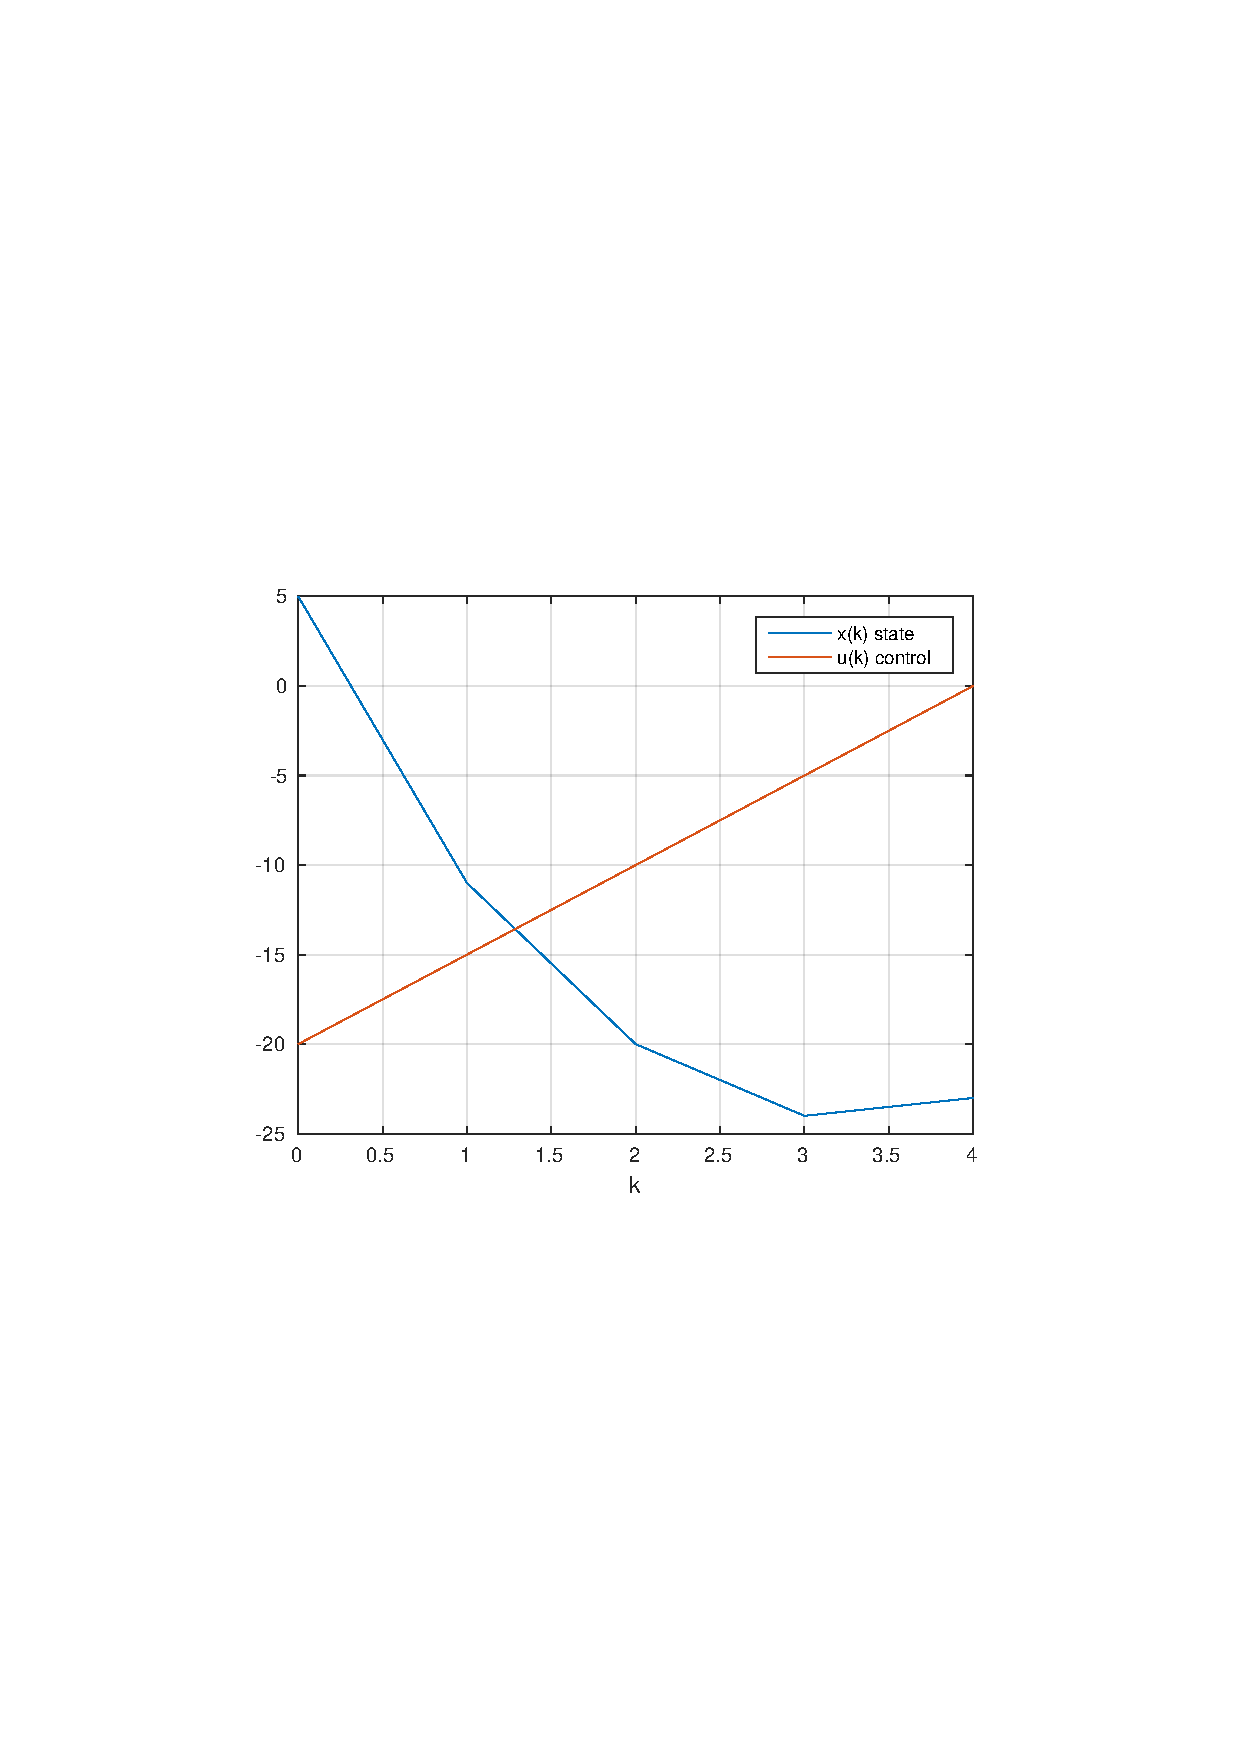
\includegraphics[width=0.6\textwidth, trim=4cm 9cm 4cm 10cm, clip]{mm3.pdf} %left bottom right top
  \caption{Shows the optimisation of the state and the corresponding control}
  \label{fig:opti}
\end{figure}
